\cleardoublepage                                   
\chapter{Agente de Carga (AC)}

\section{Hardware}

%---------------------------------------descripción general del hardware---------------------------------------
El AC está implementado sobre una placa de desarrollo basada en un microcontrolador ESP32 de 32 bits. La elección de esta plataforma responde a su adecuada capacidad de procesamiento e interfaces para las tareas requeridas, su amplia disponibilidad en el mercado junto a un bajo costo y la extensa base de recursos técnicos existentes, lo que facilita su programación y mantenimiento. Este dispositivo integra las funciones de adquisición de datos, cálculo de variables eléctricas y comunicación tanto con la microrred como con los NC.

El sistema cuenta en primer lugar con una etapa de alimentación encargada de acondicionar la tensión de corriente alterna proveniente de la microrred para energizar el circuito completo. La estabilidad de esta fuente es fundamental, ya que variaciones significativas en su salida introducen errores en las mediciones realizadas por el AC o pueden afectar el desempeño del microcontrolador.

Para la medición de la tensión de la microrred se emplea un módulo sensor basado en el transformador de señal ZMPT101B, seleccionado tanto por sus características técnicas como por su disponibilidad comercial. Este módulo genera una señal sinusoidal con un nivel de continua (offset) y una amplitud proporcional a la tensión real medida. Antes de ser leída por la entrada analógica del microcontrolador, la señal atraviesa una etapa de adecuación que garantiza que sus valores se mantengan dentro del rango permitido por el ESP32, evitando sobrepasar el límite máximo de 3,3 V.

Con el fin de comunicarse con los demás agentes que intervienen en la microrred, el AC incorpora un módulo CAN basado en el controlador MCP2515. Este dispositivo actúa como interfaz física entre el microcontrolador y el bus diferencial del protocolo CAN, permitiendo tanto el envío como la recepción de mensajes. El módulo se conecta al ESP32 mediante la interfaz SPI, a través de la cual se gestionan las señales de control (CS, INT) asociadas a la transmisión y recepción de datos.

El intercambio de información entre el AC y los NC se complementa mediante el protocolo inalámbrico ESP-NOW, soportado nativamente por el ESP32. Este protocolo opera en la banda Wi-Fi pero utiliza directamente la capa de enlace de datos. Al prescindir de redes Wi-Fi existentes, encabezados adicionales y procesos de reensamblado, ofrece baja latencia y alta confiabilidad en enlaces de corto a mediano alcance.

En virtud de la naturaleza distribuida del sistema, el AC también actúa como receptor de los datos de consumo enviados por todos los NC. Estos valores, junto con los parámetros globales de consumo y generación de la microrred que el propio AC calcula, son transmitidos mediante una interfaz UART a un módulo ESP32-S3 Super Mini. Este módulo tiene como función publicar la información recibida en un servidor externo para su almacenamiento, visualización y análisis posterior, permitiendo así integrar la operación local de la microrred con herramientas remotas de supervisión.

Finalmente, el AC incorpora una interfaz local destinada a la interacción con el usuario. Esta incluye un display que proporciona retroalimentación visual inmediata y que se comunica con el microcontrolador mediante la interfaz serie I²C. Se integran además pulsadores que permiten navegar entre distintas pantallas e ingresar parámetros operativos del Sistema de Gestión de Consumo (SGC), facilitando su configuración y supervisión sin necesidad de herramientas externas.

%---------------------------------------descripción del diseño PCB---------------------------------------
Pensando en la integración del AC dentro de instalaciones eléctricas ya existentes, se consideró fundamental que su montaje no requiriera intervenciones complejas ni modificaciones significativas de la infraestructura del usuario. En entornos residenciales, comerciales e industriales es habitual la presencia de cajas de paso estandarizadas de 10×10 cm, ampliamente utilizadas en canalizaciones eléctricas convencionales. Con el fin de favorecer la compatibilidad con este tipo de cajas y facilitar su incorporación por parte de instaladores de sistemas de microrredes, el diseño de la placa de circuito impreso (PCB) del AC se desarrolló teniendo en cuenta esta restricción dimensional desde el inicio del proceso.

La PCB se definió para ajustarse al espacio interno de la caja mencionada, respetando las distancias necesarias para acomodar todos los componentes que forman parte del circuito, la separación entre zonas de baja tensión y las partes asociadas a la medición de la tensión del bus y la fuente de alimentación. En base a estas consideraciones se organizaron los componentes siguiendo una disposición que permitiera mantener recorridos cortos en la medida de lo posible para las señales sensibles como, por ejemplo, la adquisición de la tensión, asegurar una correcta disipación térmica y reservar ubicaciones accesibles para conectores, borneras y elementos de interfaz con el usuario.

El diseño final del PCB, mostrado en los Anexos~\ref{anx:esquematico-pcb-nc}, refleja estas decisiones, integrando en un espacio compacto todos los elementos funcionales del AC y permitiendo su instalación en una caja de paso estándar sin requerir adaptadores adicionales. Esta compatibilidad busca facilitar significativamente su implementación, reduciendo tiempos y costos de instalación y contribuyendo a que el sistema pueda ser incorporado como un módulo más dentro de las soluciones habituales manejadas por empresas instaladoras de sistemas de paneles solares.

%---------------------------------------descripción del armado---------------------------------------
En cuanto al proceso de fabricación del prototipo, el mismo se realizó en base técnicas accesibles que permitieran validar el funcionamiento del AC antes de avanzar hacia una producción más estandarizada. La PCB fue elaborada mediante el método de transferencia, técnica ampliamente utilizada en etapas iniciales de desarrollo por su bajo costo y rapidez de implementación. Una vez transferido el diseño al cobre y completado el proceso de grabado mediante la reacción química de oxidación-reducción con cloruro férrico, se realizaron las perforaciones necesarias para la colocación de los componentes, conectores y módulos externos. Posteriormente, se llevó a cabo el montaje y la soldadura de todos los elementos, asegurando una correcta fijación mecánica y verificando la continuidad eléctrica en cada etapa.

Con el objetivo de integrar la interfaz local en la caja de paso de 10×10 cm, se efectuó un mecanizado de la tapa para alojar tanto los pulsadores como el display. La disposición de estos elementos fue seleccionada para garantizar accesibilidad al usuario, buena visibilidad y comodidad durante la utilización del sistema. Para asegurar un montaje firme y estético del display, se diseñó un soporte específico mediante software de modelado tridimensional y se imprimió en 3D utilizando material plástico de alta resistencia. Este soporte permite fijar el display en la posición adecuada y facilita el ensamblaje final sin necesidad de herramientas adicionales.

El conjunto resultante, mostrado en la Figura~\ref{img:ac}, combina una PCB que cumple con las restricciones de diseño y una interfaz accesible en un dispositivo práctico para la instalación en una infraestructura existente.


\begin{figure}[hbt!]
    \centering
    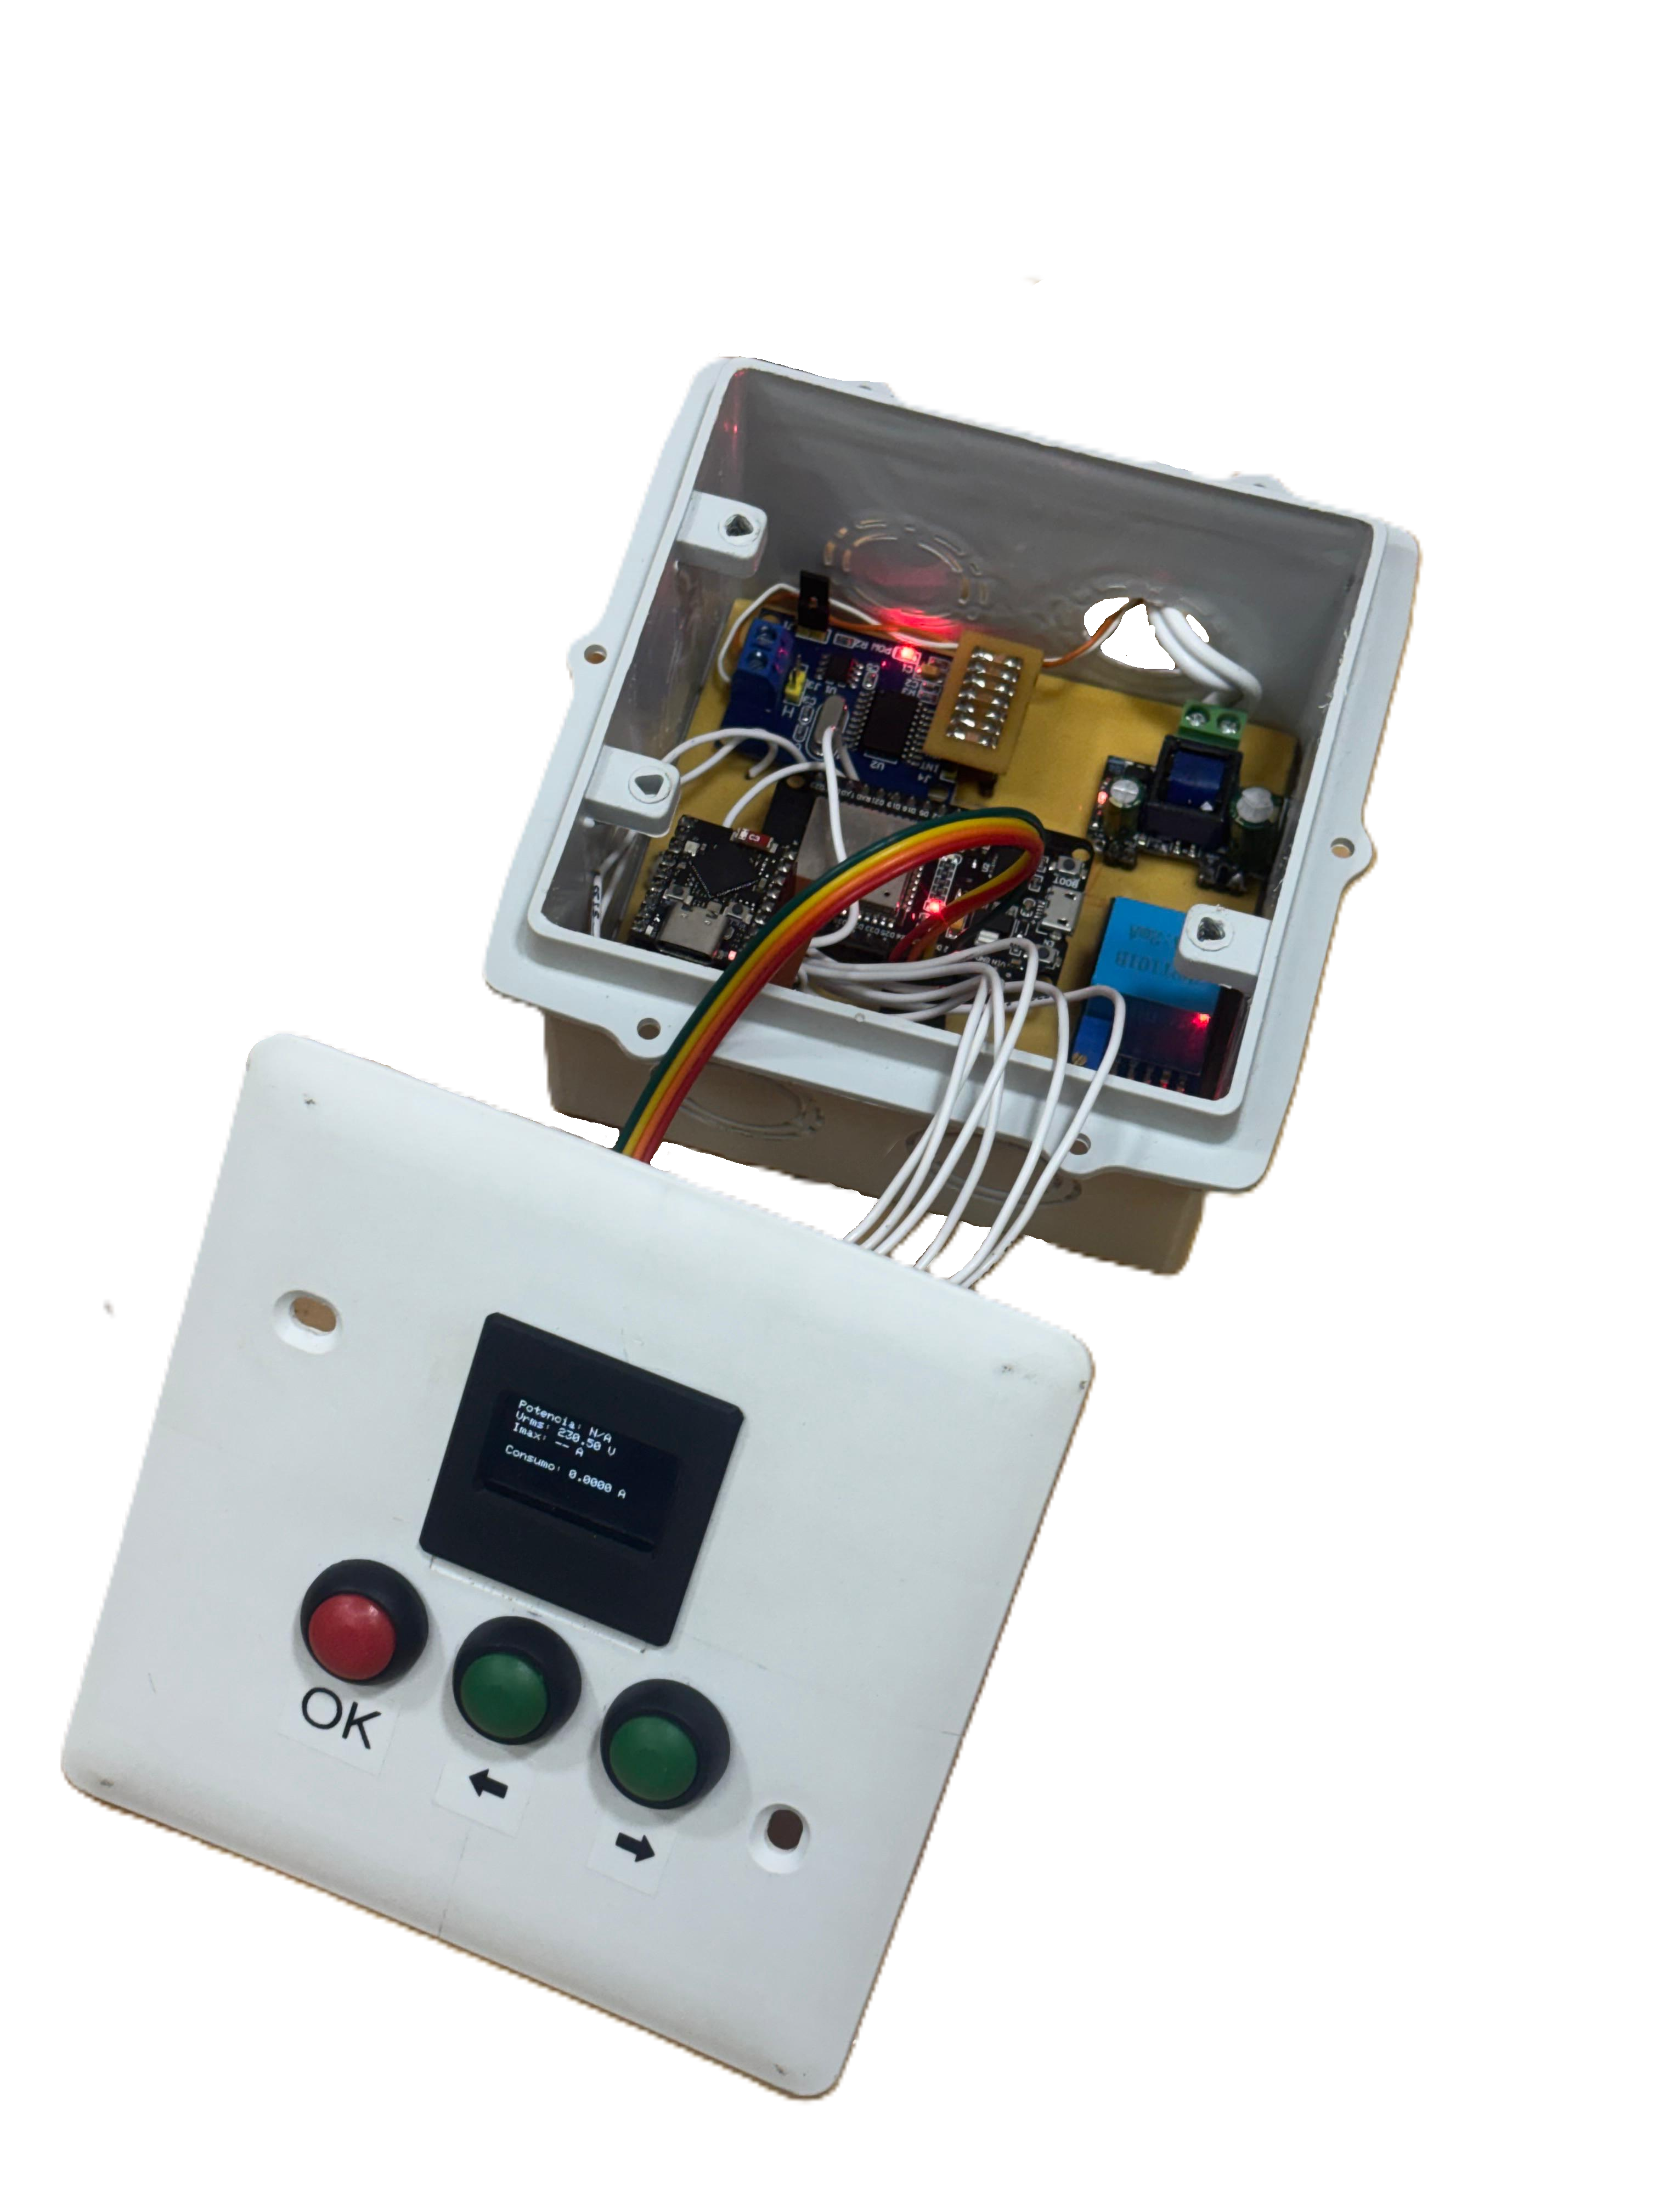
\includegraphics[width=0.6\textwidth]{imagenes/ac.jpg}
    \caption{Hardware desarrollado para el Agente de Carga(AC)}
    \label{img:ac}
\end{figure}

\section{Firmware}

El desarrollo del firmware para el AC se basó en una arquitectura cooperativa de tiempo real, diseñada para garantizar la integridad de las mediciones eléctricas sin sacrificar la capacidad de respuesta en las comunicaciones. La estructura del código separa las tareas críticas de baja latencia, como el muestreo de señales, de las tareas de gestión de alto nivel, como la actualización del display y el manejo de los protocolos de red.

Las funciones de alta prioridad, específicamente la lectura del conversor analógico-digital (ADC) y los temporizadores del microcontrolador, se ejecutan de inmediato gracias a rutinas de servicio de interrupción (ISR). Por otro lado, la lógica de control principal, que incluye el envío y recepcion de mensajes CAN, la gestión de la red ESP-NOW y la interfaz de usuario, se procesa en el bucle principal (main loop) de manera no bloqueante. Esta separación asegura un comportamiento determinista en la adquisición de datos, evitando que el procesamiento de las comunicaciones degrade la precisión de la medición de tensión.

\subsection{Adquisición y Procesamiento de Señales}

La medición de la tensión de línea proveniente de la microrred se realiza mediante un muestreo síncrono de alta frecuencia. Se configuró un temporizador por hardware para generar interrupciones a una frecuencia de 50 kHz. En cada interrupción, se dispara la conversión del ADC, asegurando que la frecuencia de muestreo sea un múltiplo exacto de la frecuencia fundamental de la red (50 Hz). Esto permite capturar un número entero de periodos de la señal, minimizando el error por efecto de ``ventaneo'' en el cálculo del valor eficaz (RMS).

El firmware implementa un procedimiento de calibración al inicio para determinar el nivel de continua (offset) introducido por el sensor ZMPT101B. Posteriormente, en tiempo de ejecución, cada muestra es corregida restando este offset. El valor RMS se calcula procesando la suma de los cuadrados de las muestras adquiridas en una ventana de tiempo definida, aplicando luego la raíz cuadrada según la Ecuación~\ref{eq:rms}:

\begin{equation}
    V_{rms} = \sqrt{\frac{1}{N} \sum_{n=0}^{N-1} (v[n] - V_{offset})^2} \times K_{sens}
    \label{eq:rms}
\end{equation}

Donde $N$ es el número total de muestras en la ventana de medición, $v[n]$ es el valor digital de la muestra actual, $V_{offset}$ es el valor de calibración de cero y $K_{sens}$ es el factor de sensibilidad del hardware. Este valor de tensión eficaz, combinado con la potencia disponible informada por el sistema de supervisión, permite al AC determinar la corriente máxima que puede ser consumida por el conjunto de cargas.

\subsection{Gestión de Comunicaciones}

El AC actúa como un puente de información, gestionando dos dominios de comunicación simultáneos: el enlace cableado con la supervisión de la microrred y la red inalámbrica con los NC.

\subsubsection{Bus CAN (Integración con la Microrred)}
La comunicación con los demás agentes de supervisión de la microrred se realiza a través del bus CAN. La lógica de transmisión implementada es no bloqueante: el AC intenta enviar sus reportes de estado y, en caso de fallo, realiza un número limitado de reintentos. El sistema cuenta con un mecanismo de recuperación de fallos que monitorea los errores de transmisión; si estos superan un umbral predefinido, el firmware reinicia automáticamente el controlador MCP2515 para restablecer el servicio sin intervención del usuario.

Para verificar el correcto funcionamiento de la capa física y la lógica de transmisión, se realizaron pruebas conectando el AC a un módulo analizador de bus CAN vinculado a una computadora. Como se observa en la Figura~\ref{img:prueba-can}, esto permitió visualizar en tiempo real los paquetes inyectados en el bus por el AC, confirmando la correcta estructura de los identificadores y los datos enviados antes de la integración final con los demás agentes.

\begin{figure}[H]
    \centering
    \includegraphics[width=0.7\textwidth]{imagenes/prueba-busCAN.png}
    \caption{Prueba de comunicación vía bus CAN entre el AC y el sistema de supervisión de la microrred}
    \label{img:prueba-can}
\end{figure}

\subsubsection{Red ESP-NOW (Gestión de Cargas)}
Para la coordinación con los NC, el firmware gestiona el intercambio de mensajes de control sin conexión (connectionless). El AC difunde periódicamente un mensaje de \textit{Disponibilidad}, que contiene el límite de corriente calculado para la red. A su vez, se mantiene a la escucha de los mensajes de \textit{Consenso} provenientes de los nodos, los cuales reportan su consumo actual y prioridad.

La gestión de la lista de nodos es dinámica: al recibir un mensaje de un NC, el AC actualiza su registro interno o lo añade si es un nodo nuevo. Para mantener la coherencia del sistema, el firmware ejecuta una rutina de limpieza que elimina de la lista a aquellos nodos que no han reportado actividad tras un periodo de tiempo determinado (timeout), evitando así que datos obsoletos afecten el cálculo del consumo total.

\subsubsection{UART (Gateway)}
Adicionalmente, el AC consolida toda la información anterior y la transmite vía UART hacia el módulo secundario (ESP32S3-SuperMini), encargado de la publicación de datos via MQTT hacia la plataforma IoT, liberando al procesador principal de las tareas de conexión Wifi y publicacion de datos hacia el broker.

\subsection{Interfaz de Usuario}

La interacción local se gestiona mediante la actualización condicional del display OLED. Para minimizar la carga de procesamiento, el contenido de la pantalla solo se redibuja cuando se detectan cambios significativos en los valores mostrados o cuando el usuario interactúa con los pulsadores.

La Figura~\ref{img:ac-pantalla} muestra la pantalla principal de operación, donde el usuario puede visualizar en tiempo real las variables críticas del sistema: la potencia disponible ($P_{disp}$), la tensión eficaz de red ($V_{rms}$), la corriente máxima calculada ($I_{max}$) y el consumo actual del sistema ($I_{cons}$). El firmware también incluye pantallas de diagnóstico para verificar el estado del bus CAN y listar los nodos conectados.

\begin{figure}[H]
    \centering
    \includegraphics[width=0.2\textwidth]{imagenes/ac-pantalla.png}
    \caption{Pantalla implementada para el AC. Muestra los valores de tensión, potencia y corriente disponibles en la microrred.}
    \label{img:ac-pantalla}
\end{figure}